\section{Food Webs}

    \begin{figure}[H]
        \centering
        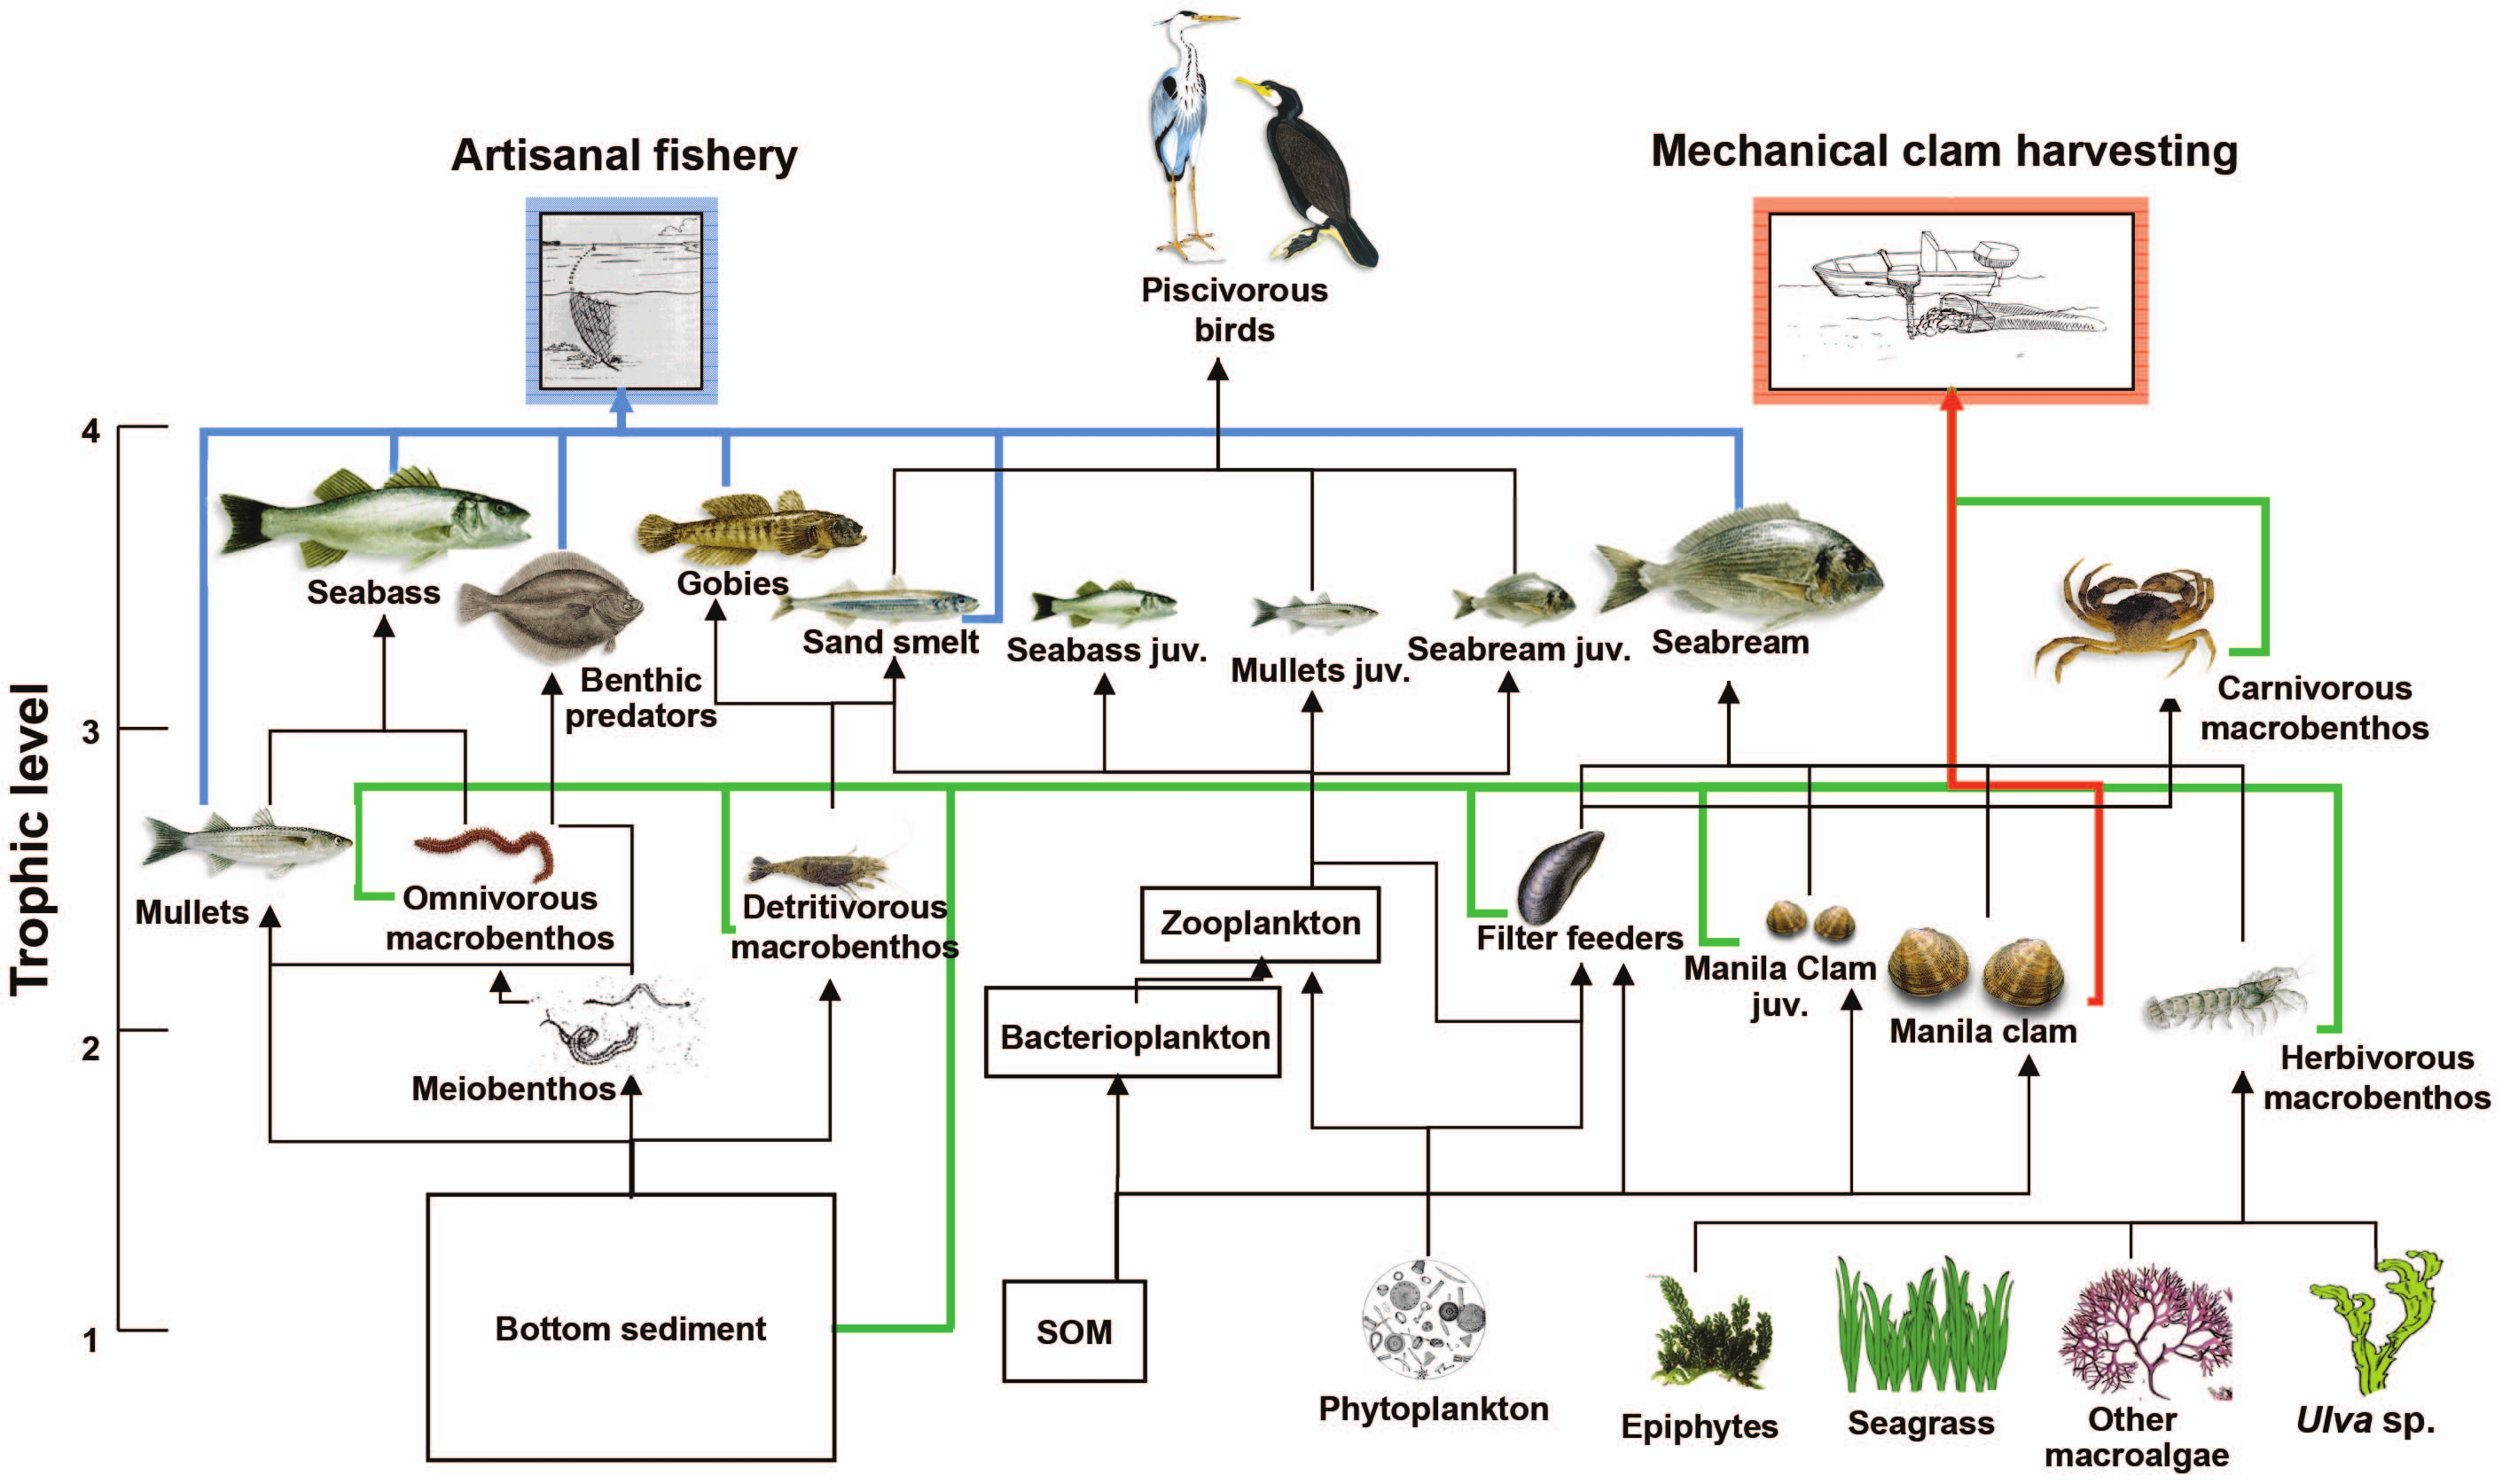
\includegraphics[width=0.9\textwidth]{images/GEN-009.png}

        \caption{Food web diagram of the Venice lagoon. From: \cite{heymans}.}
        \label{fig:food-web}
    \end{figure}

    One of the most common networks used in school comes from biology, the food webs. Here, the nodes usually are species in a given ecological community (Venice lagoon, for \cref{fig:food-web}) and the links map the feeding connection between the species, which species feeds on another.
